%!TEX TS-program = xelatex
%!TEX encoding = UTF-8 Unicode

\documentclass[11pt,tikz,border=1]{standalone}
\usepackage{pgfplots}
\usetikzlibrary{positioning}

\begin{document}
  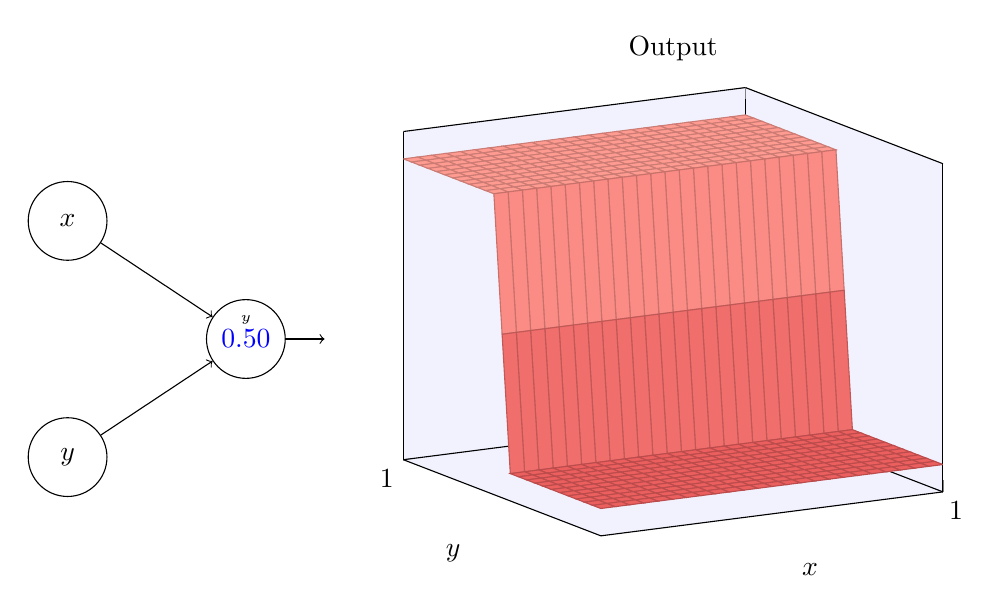
\begin{tikzpicture}[
    neuron/.style={circle,draw,inner sep=0pt,minimum size=10mm}
    ]
    
    \begin{scope}
      \node(n) [neuron] {};
      \node(x) [neuron,left=1.25 of n,yshift=1.5cm] {$x$};
      \node(y) [neuron,left=1.25 of n,yshift=-1.5cm] {$y$};
    
      \draw[->] (x) to (n);
      \draw[->] (y) to (n);
  
      \node (s) [blue] at (n.center) {$0.50$};
      \node at (s.north) {\tiny $y$};
      
      \draw[->] (n) -- ++(1cm, 0);
    \end{scope}
    
    \begin{scope}[xshift=2cm,yshift=-2.5cm]    
      \begin{axis}[
        view={-30}{15},        
        axis background/.style={fill=blue!5},
        xlabel=$x$,
        ylabel=$y$,
        xtick distance=1,
        ytick distance=1,
        ztick distance=1,
        xtick={1},
        ytick={1},
        ztick={2},
        title=Output,
        colormap={simple}{rgb255=(235,95,95) rgb255=(255,155,145)}
        ]
        \addplot3[surf,domain=0:1] {
          1 / (1 + exp(-(1000) * y - (-0.5 * 1000)))
        };
      \end{axis}
    \end{scope}
    
  \end{tikzpicture} 
\end{document}
